\section{}

\subsection*{Propagation of errors}

If we measure a value \(x\) then we call the uncertainty in this measurement \(\delta x\). We give the result as \(x\pm\delta x\). If \(y=f(x)\) then by plotting the function evaluating at \(x,x+\delta x\) and \(x-\delta x\) it can be shown that an there is an error range either side of the calculated value of \(y\). We assume that the error on both sides of \(y\) is the same and we call it \(\delta y\). We assume that the error is small enough that the function can be approximated as a straight line
\[\therefore \frac{\delta y}{\delta x}=\text{gradient}=\frac{dy}{dx}\]
\[\implies\delta y=\frac{dy}{dx}\biggr|_x\delta x\]
\[\implies y\pm\delta y=f(x)\pm\frac{dy}{dx}\biggr|_x\delta x\]
For a multivariable function such as \(w=f(x,y,z)\) where \(x,y\) and \(z\) have uncorrelated errors (errors that don't effect eachother) we write the contribution of \(x\) to the error of \(w\) as \(\delta w_x\). It is calculated as:
\[\delta w_x=\pd wx\biggr|_x\delta x\]

We combine the errors by adding errors in quadrature. That is each error is squared and then added together and squarerooted:
\[\delta w=\sqrt{\delta w_x^2+\delta w_y^2+\delta w_z^2}\]

\part{Waves}
\section{}

A wave is anything that satisfies the wave equation. It is a function of poition in space \(x\) and time \(t\). The displacement of part of the medium distance \(x\) from the source at time \(t\) is given by \(y(x,t)\) where function \(y\) is a solution to the wave equation:
\begin{center}
\boxed{\pd[2]yt=v^2\pd[2]yx}
\end{center}

This is an idealised equation. In reality only light in a vacuum follows this. One solution to the wave equation is:
\[y(x,t)=f(x\pm vt)\]
A particularly common form is:
\[y(x,t)=A\sin(kx\pm\omega t+\varphi)\]
The \(\pm\) represents the two directions the waves can go in. If it is a \(+\) then the wave travels in the negative \(x\) direction. If it is a \(-\) then the wave travels in the positive \(x\) direction. \(A\) is the amplitude or maximum displacement of the wave. \(k\) is how much the wave changes with space and \(\omega\) is how much the wave changes with time. \(\varphi\) is the phase difference. Some common wave properties can be calculated as follows:
\[\lambda=\frac{2\pi}{k},\quad T=\frac{2\pi}{\omega}\quad\text{ and }\quad f=\frac{\omega}{2\pi}=\frac 1T\]
The units of \(f\) and \(\omega\) are \si{s^{-1}} and \si{rad.s^{-1}} respectively, both of these are the same as \si{s^{-1}} and \si{Hz}. The units of \(k\) are \si{rad.m^{-1}} which is the same as \si{m^{-1}}. The units of \(x\) and \(y\) are \si{m} and the units of \(t\) are \si{s}.

A node is anywhere where \(y(x,t)=0\). For the example with the sine function since \(\sin t=0\,\A t\in\{n\pi|n\in\bb Z\}\). If the \(n^{\text{th}}\) node is at \(x_n\) then:
\begin{align*}
kx_n-\omega t&=n\pi\\
kx_0-\omega t&=0\\
kx_0&=\omega t\\
\frac{x_0}{t}&=\frac{\omega}{k}=v\\
v&=\frac{2\pi f}{\frac{2\pi}{\lambda}}=f\lambda
\end{align*}

The wave speed depends on the medium not the source:
\[v^2=\frac{\text{stiffness}}{\text{inertia}}\]
The wave speed can also depend on frequency. If frequency doesn't effect wavespeed then we say the wave is dispersionless. 

The speed that any one part of the medium is moving \(u\), is given by:
\[u=\pd yt=\frac{\partial}{\partial t}(A\sin(kx-\omega t+\varphi))=-\omega A\cos(kx-\omega t+\varphi)\]

\subsection*{Doppler shift}

\begin{center}
\includegraphics[scale=0.4]{Doppler}
\end{center}

The wavespeed is \(v\) and the source is moving at speed \(v_s\). In this equation \(n'\) means \(n\) after the doppler shift is taken into account. At \(t=0\) the first peak of the wave is emitted. At time \(t=T\) the second peak is emitted. In the time between peaks the first peak has moved distance \(x_1=vT\) and the source has moved distance \(x_2=v_sT\). The distance between the two peaks is:
\[\lambda'=x_1-x_2=vT-v_sT=T(v-v_s)\]
The original wavelength \(\lambda\):
\[\lambda=vT\implies T=\frac{\lambda}{v}\implies\lambda'=\lambda\frac{v-v_s}{v}\]
Finally substituting for \(f\):
\[v=f\lambda\implies\lambda=\frac vf\implies f'=f\frac{v}{v-v_s}\]
As \(v_s\to v\) we get a sonic boom. If both the source and detector are moving and the detector speed is \(v_d\) then the same logic can lead to the equation:
\[f'=f\left(\frac{v\pm v_d}{v\pm v_s}\right)\]
The \(\pm\) is just dependant on the relative directions of the speeds, just think about whether the frequency should increase (source and detector coming together) or decrease (source and detector seperating).
 
\section{}

Linearity is a property of some systems. If \(x\) and \(y\) are solutions to the system then \(x+y\) is also a solution to the system. Differentiation is a linear operator, that is:
\[\diff[2] x(f(x)+g(x)=f'(x)+g'(x)\]

The wave equation is also linear so if \(y_1(x,t)\) and \(y_2(x,t)\) are solutions to the wave equation so is \(y_1+y_2\)

If \(n\) waves are present then the resulting wave is given by:
\[y(x,t)=y_1(x,t)+y_2(x,t)+\cdots y_n(x,t)=\sum_{i=1}^ny_i(x,t)\]

You must take into account the phase difference when you do this calculation.

\subsection*{Example 5.1}

Two waves that are the same but out of phase:
\[y_1(x,t)=A\sin(kx-\omega t),\quad\&\quad y_2=A\sin(kx-\omega t+\varphi)\]
\begin{align*}
y&=y_1+y_2\\
&=A\sin(kx-\omega t)+A\sin(kx-\omega t+\varphi)\\
&=A(\sin(kx-\omega t)+\sin(kx-\omega t+\varphi)\\
\intertext{There is a useful trig identity for this: \(\sin\alpha+\sin\beta=2\sin\left(\frac{\alpha+\beta}{2}\right)\cos\left(\frac{\alpha-\beta}{2}\right)\)}
y&=2A\sin\left(\frac{kx-\omega t+kx-\omega t+\varphi}{2}\right)\cos\left(\frac{kx-\omega t-kx+\omega t-\varphi}{2}\right)\\
&=2A\sin\left(kx-\omega t+\frac{\varphi}{2}\right)\cos\left(\frac{\varphi}{2}\right)\\
&=2A\cos\left(\frac{\varphi}{2}\right)\sin\left(kx-\omega t+\frac{\varphi}{2}\right)
\end{align*}
The new wave that is formed now has amplitude \(2A\cos\left(\frac{\varphi}{2}\right)\) and is \(\frac{\varphi}{2}\) \si{rad} out of phase.

\subsection*{Example 5.2}

Two waves that are the same but traveling in opposite direction:
\[y_1(x,t)=A\sin(kx-\omega t),\quad\&\quad y_2=A\sin(kx+\omega t)\]
\begin{align*}
y&=y_1+y_2\\
&=A\sin(kx-\omega t)+A\sin(kx+\omega t)\\
&=A(\sin(kx-\omega t)+\sin(kx+\omega t)\\
&=2A\sin\left(\frac{kx-\omega t+kx_\omega t}{2}\right)\cos\left(\frac{kx-\omega t-kx+\omega t}{2}\right)\\
&=2A\sin(kx)\cos(\omega t)
\end{align*}
\(\sin(kx)\) is spatial oscillation. \(cos(\omega t)\) is time oscillation.

This is what happens to produce standing waves. A standing wave doesn't move, that means that no energy is transfered. A node is anywhere where \(y(x,t)=0\A x,t\), nodes don't move.

To solve a differential equation you must know the boundary conditions eg. position or speed of the wave at a given time or what is causing the wave. 

\subsection*{Example 5.3}

A standing wave is set up in a string length \(L\) fixed at both ends. What are the boundary conditions of the system?

Since the ends of the string are at positions \(x=0,L\) and they are fixed \((y=0)\) we know that \(y(0,t)=y(L,t)=0\A t\).

We know that \(y(x,t)=2A\sin(kx)\cos(\omega t)\). We need \(\sin(kx)=0\) for \(x=0,L\implies kx=n\pi\, n\in\bb Z,\,n\ne0\implies KL=n\pi\). Substituting in \(k=\frac{2\pi}{\lambda}\) gives \(\lambda=\frac{2L}{n}\)

The longest wavelength \((n=1)\) is the ``fundamental". All shorter wavelengths are ``harmonics". Physical systems usually give a mix of harmonics. Any pattern on the string can be made from a combination of sine nodes.

\subsection*{Example 5.4}

Two waves with different frequencies:

When this occurs the beats phenomonem can be observed, this is the reason that two slightly out of tune notes have a slightly oscillating pitch.

\[y_1(x,t)=A\sin(kx-\omega_1 t),\quad\&\quad y_2=A\sin(kx+\omega \_2t)\]
\begin{align*}
y&=y_1+y_2\\
&=A\sin\left(kx-\omega_1 t\right)+A\sin\left(kx+\omega \_2t\right)\\
&=A(\sin\left(kx-\omega_1t\right)+\sin\left(kx-\omega_2t\right))\\
&=2A\sin\left(\frac{kx-\omega_1t+kx-\omega_2t}{2}\right)\cos\left(\frac{kx-\omega_1t-kx+\omega_2t}{2}\right)\\
&=2A\sin\left(kx-\frac{\omega_1+\omega_2}{2}\right)\cos\left(\frac{\omega_2-\omega_1}{2}t\right)\\
&=2A\sin\left(kx-\bar{\omega}\right)\cos\left(\frac{\Delta \omega}{2}t\right)
\end{align*} 
Where the mean angualr frequency \(\bar\omega=\frac{\omega_1+\omega_2}{2}\) and the difference in angular frequencies \(\Delta\omega=\omega_2-\omega_1\)

\section{}

James Clerk Maxwell showed that light was a wave that followed the following vector calculus:
\[\nabla\cdot\vv E=\frac{\rho}{\varepsilon_0}\]
\[\nabla\cdot\vv B=0\]
\[\nabla\times\vv E=-\vv B\]
\[\nabla\times\vv B=\mu_0(\vv J+\varepsilon_0)\]

From this we can derive wave equations for \(\vv E\) and \(\vv B\). In 1D the equations are:
\[\pd[2]{E}{t}=\frac{1}{\mu_0\varepsilon_0}\pd[2]{E}{x}\]
\[\pd[2]{B}{t}=\frac{1}{\mu_0\varepsilon_0}\pd[2]{B}{x}\]
From this equation we get:
\[v=c=\frac{1}{\sqrt{\mu_0\varepsilon_0}}=\SI{299792458}{m.s^{-1}}\]
A light wave is made of perpendicular waves in the electromagnetic field. The light can be polarised and it can rotate along its axis of travel but the waves always remain perpendicular.

Thomas Young's double slit experiment showed light interfering with itself which is wave behaviour.

Light is not a wave or a particle. It is a quantum object with properties of a wave and a particle. There is no intuitive picture analagous to something that we can see.

We can't see the oscillations of light with time as our eyes don't react fast enough. What we see is the time average of the square of the wave amplitude. That is the time average of the energy of the wave \((E\propto A^2)\).

\subsection*{Light intensity of a sinusoidal wave}

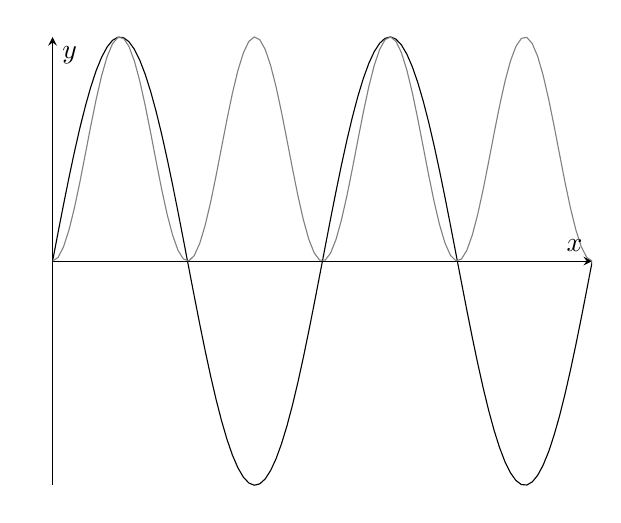
\begin{tikzpicture}
\begin{axis}[
    axis lines = left,
    axis lines = center,
    xtick style={draw=none},
    ytick style={draw=none},
    xticklabels={},
    yticklabels={},
    xlabel = $x$,
    ylabel = {$y$},
]

\addplot [
    domain=0:12.566, 
    samples=100, 
    color=black,
]
{sin(deg(x))};


\addplot [
    domain=0:12.566, 
    samples=100, 
    color=gray,
    ]
    {(sin(deg(x)))^2};

 
\end{axis}
\end{tikzpicture}

This graph shows \(y=\sin x\) and \(y=\sin^2x\).

The intensity \(I\) is given by \(I=\langle|y|^2\rangle_t\) where \(\langle p\rangle_q\) is the average of \(p\) as \(q\) varies.
\[I=\frac 1t\int_0^Ty^2\,dt\]
Here the integral is like taking the mean of a continuous function rather than the discrete data you would usually take the mean of.
\[y=A\sin(\omega t)\]
\[y^2=A^2\sin^2(\omega t)\]
\[I=\frac 1T\in_0^TA^2\sin^2(\omega t)\,dt\]
\[I=\frac{A^2}{T}\left[\frac t2-\frac 14\sin(2\omega t)\right]_0^T\]
At \(t=nT\) for \(n\in\bb Z\) \(\sin(2\omega nT)=\sin(2m\pi)=0\) for \(m\in\bb Z\)
\[I=\frac{A^2}{2}\]
\[I\propto A^2\]

A prisim can split white light showing that it is composed of all other frequencies of visible (and some non-visible) light.

Real instruments (including our eyes) are sensitive to specific wavelength ranges
\[R=\int s(\lambda)I(\lambda)\,d\lambda\]
Where \(R\) is the recieved signal, \(s(\lambda)\) is the sensitivity function and \(I(\lambda)\) is the incoming intensity.

\subsection*{Dispersion}

A pulse of light is made of lots of frequencies of wave together. In free space (a vacuum) all of these travel at the same speed. In any other medium they all travel at different speeds.

The peaks of each frequency travel at a different speed to the whole packet. We call the speed of the individual frequencies the phase velocity, \(v_p\) and the speed of the whole packet the qroup velocity, \(v_g\).

In free space light travels at \(c\). In a medium with refractive index \(n\) light travels at \(\frac cn\) \((n>1)\). In this case \(\omega=ck\) isn't always true. Media have a dispersion relation \(\omega(k)\):
\[v_p=\frac{\omega}{k}\quad\&\quad v_g=\pd{\omega}{k}=\pd{\omega(k)}{k}\]
Often but not always for light \(v_pv_g=c^2\) and \(v_p\ge c,v_g\le c\). It is ok for \(v_p>c\) as no information is being transferred.

In a plasma (ionised gas) free electrons interact with the electromagnetic field giving:
\[\omega=\frac{ck}{\sqrt{1-\frac{\omega_0^2}{\omega^2}}}\]
\[v_p=\frac{\omega}{k}=\frac{c}{\sqrt{1-\frac{\omega_0^2}{\omega^2}}}\]
Note that, for some values of \(\omega\), \(v_p\not\in\bb R\) This is what happens in opaque objects.

\section{}

\[v_g=\pd{\omega}{k}\]
\[\omega=\frac{ck}{\sqrt{1-\frac{\omega_0^2}{\omega^2}}}\]
\[\omega^2=\frac{c^2k^2}{1-\frac{\omega_0^2}{\omega^2}}\]
\[\omega^2\left(1-\frac{\omega_0^2}{\omega^2}\right)=c^2k^2\]
\[\omega^2-\omega_0^2=c^2k^2\]
\[\omega^2=\omega_0^2+c^2k^2\]
\[\omega=\sqrt{\omega_0^2+c^2k^2}\]
\[v_g=\pdiff{k}\left(\omega_0^2+c^2k^2\right)^{-\frac{1}{2}}\]
\[=\frac{c^2k}{\sqrt{\omega_0^2+c^2k^2}}\]

\subsection*{Geometric optics}

Geometric optics is an approximation of light to linear rays travelling in the same direction as the wave.

When light enters a medium it changes speed so that (group) speed is equal to \(v=\frac cn\) where \(n\) is the refractive index of the material. \(n>1\) for all media. \(n=1\) for a vacuum and \(n\approx1\) for air. When light travels across a boundary it can either reflect or refract. Usually it does a combination of both. It depends on the properties of the medium, the light path and the frequency as to what occurs.

\subsection*{Reflection mechanis}

When a light ray is incident on a surface it causes free electrons accelerate which causes them to emit EM radiation which cancels with some waves and not others resulting in only the reflected wave leaving the medium. If the new medium has a higher refractive index then the reflected wave has a phase shift of \(\SI{\pi}{rad}\). If the new medium has a lower refractive index then there is no phase change.

Specular reflection occurs on smooth surfaces with lots of free electrons (metals). Specular reflections preserve the image. Disperse reflections occur in all other cases, usually because at a small enough scale the surface is not flat.

\subsection*{Law of reflection}

\begin{itemize}
\item The incident ray, reflected ray and surface normal are all in the same plane.
\item The angle of incident is the same as the angle of refelection \(\vartheta_i=\vartheta_r\)
\end{itemize}

\begin{center}
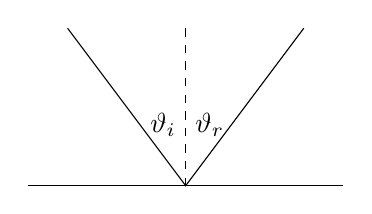
\begin{tikzpicture}[scale=1]
\draw (0,0) -- (4,0);
\draw [dashed] (2,2) -- (2,0);
\draw (0.5,2) -- (2,0) -- (3.5,2);
\node [above left] at (2,0.5) {\(\vartheta_i\)};
\node [above right] at (2,0.5) {\(\vartheta_r\)};
\end{tikzpicture}
\end{center}

\subsection*{Refraction}

\begin{center}
\begin{tikzpicture}
\draw (-4,-2) -- (4,-2) -- (4,2) -- (-4,2) -- (-4,-2);
\draw [ultra thick] (0,2) -- (0,-2);
\draw [dashed] (-4,0) -- (4,0);
\draw (-3,-1) -- (0,0) -- (3,0.5);
\node [below]  at (-2,-2) {\(n_1\)};
\node [below] at (2,-2) {\(n_2\)};
\node [below left] at (-1.2,0) {\(\vartheta_1\)};
\node [above right] at (2,-0.1) {\(\vartheta_2\)};
\end{tikzpicture}
\end{center}

When light passes from an optically less dense to optically more dense material it bends towards the normal and vice versa.

\subsection*{Snell's law}

\[n_1\sin\vartheta_1=n_2\sin\vartheta_2\]

\subsection*{Fermat's principle}

The path taken by light minimise the travel time. (Note that it is a local minimum not a global minimum)

If we define path length \(l=nd\) where \(d\) is the distance travelled and \(n\) is the refractive index then if we have several materials we get:
\[l=\sum_id_in_i\]
and for a continuously changing material:
\[l=\int_{\text{path}}n\,ds\]
where \(ds\) is an element of the path.

The speed of light is given by \(v=\frac cn\) so the time taken to travel \(t\) is given by:
\[t=\frac dv=\frac{d}{\frac{c}{n}}=\frac{nd}{c}=\frac lc\]
From this we can see that \(t\propto l\) so Fermat's principle can be restated as light takes the shortest local path.

Note that for both definitions the paths are local minima and make physical sense.

\subsection*{Derivation of the law of reflection}

\begin{center}
\begin{tikzpicture}[scale=0.75]
\draw (0,-4) -- (0,4);
\draw (6,4) -- (0,0) -- (6,-4);
\draw [dashed] (-2,-4) -- (8,-4);
\draw [dashed] (-2,4) -- (8,4);
\draw [dashed] (-2,0) -- (8,0);
\draw [<->] (8,-4) -- (8,4);
\node [right] at (8,0) {\(y\)};
\draw [<->] (7,0) -- (7,4);
\node [right] at (7,2) {\(y_1\)};
\draw [<->] (7,0) -- (7,-4);
\node [right] at (7,-2) {\(y_2\)};
\node [above left] at (3,2) {\(d_1\)};
\node [below left] at (3,-2) {\(d_2\)};
\node [above] at (1,0) {\(\vartheta_1\)};
\node [below] at (1,0) {\(\vartheta_2\)};
\node [above right] at (6,4) {\(A\)};
\node [below right] at (6,-4) {\(B\)};
\draw [<->] (0,-4.6) -- (6,-4.6);
\draw [dashed] (0,-4) -- (0,-4.6);
\draw [dashed] (6,-4) -- (6,-4.6);
\end{tikzpicture}
\end{center}

There are two local minima in this. One has path length \(y\) and is going from \(A\) straight to \(B\) the other is to reflect off of the surface. To calculate the two angles \(\vartheta_1\) and \(\vartheta_2\) we must find the minimum distance for the light to travel:

Total distance \(D=d_1+d_2\)
By pythagoras we get:
\[d_1^2=y_1^2+x^2\quad\&\quad d_2^2=y_2^2+x^2\]
At the local minimum \(\dv{D}{y_1}=0\):
\[\dv{D}{y_1}=\frac 12\cdot2y_1(y_1^2+x^2)^{\frac 12}+\frac 12\cdot2y_2(y_2^2+x^2)^{\frac 12}\cdot\dv{y_2}{y_1}\]
\[y=y_1+y_2\implies y_2=y-y_1\]
\[\dv{y_2}{y_1}=-1\]
\[\dv{D}{y_1}=\frac{y_1}{\sqrt{y_1^2+x^2}}-\frac{y-y_1}{\sqrt(y-y_1)^2+x^2}=0\]
This is true when \(y_1=y-y_1\implies y_1=\frac 12 y\implies y_1=y_2\)
Since the lengths are equal and all angles are less than \(2\pi\) the angles \(\vartheta_1\) and \(\vartheta_2\) must be the same.

\subsection*{Derivation of Snell's law}

\begin{center}
\begin{tikzpicture}[scale=0.75]
\draw[->] (-1,0) -- (9,0);
\node [right] at (9,0) {\(x\)};
\draw[dashed]  (4,-4) -- (4,4);
\draw (0,4) -- (4,0) -- (5,-4);
\node [above] at (0,4) {\((0,y_1)\)};
\node [below] at (0,0) {\((0,0)\)};
\node [above right] at (4,0) {\((x,0)\)};
\node [above] at (8.5,0) {\(n_1\)};
\node [below] at (8.5,0) {\(n_2\)};
\node [above left] at (4.1,0.3) {\(\vartheta_1\)};
\node [below right] at (3.9,-1.8) {\(\vartheta_2\)};
\node [below] at (5,-4) {\((x_2,y_2)\)};
\node [above right] at (2,2) {\(d_1\)};
\node [right] at (4.5,-2) {\(d_2\)};
\end{tikzpicture}
\end{center}

First by the definition of \(\sin\) we get:
\[\sin\vartheta_1=\frac{x}{\sqrt{x^2+y_1^2}}\quad\&\quad\sin\vartheta_2=\frac{x_2-x}{\sqrt{(x-x_2)^2+y_2^2}}\]
\[l=n_1d_1+n_2d_2\]
\[=n_1\sqrt{(x^2+y_1^2)}+n_2\sqrt{(x-x_2)^2+y_2^2}\]
\[\dv lx=0=\frac{2xn_1}{\sqrt{x^2+y_1^2}}+\frac{2(x-x_2)n_2}{\sqrt{(x-x_2)^2+y_2^2}}\]
\[0=n_1\sin\vartheta_1-n_2\sin\vartheta_2\]
\[n_1\sin\vartheta_1=n_2\sin\vartheta_2\]

Fermat's principle can be derived from Huygen's principle that each wave front acts as a new source of waves in all directions.

\section{}

The radius of curvature of a curve is an approximation of how curved it is given by fitting a circle to part of the curve and taking the radius of the circle.

Expand the function as a taylor series:
\[y=y_0+a(x-x_0)+b(x-x_0)^2+\mathcal{O}(x^3)\]
The \(x^0\) term gives position, the \(x^1\) term gives orientation and the \(x^2\) term gives the curvature.

\begin{center}
\begin{tikzpicture}[scale=2.6]
\draw [domain=-2:2] plot (\x, {0.5*pow(\x,2)});
\draw (0,1) circle [radius=1];
\draw (0,1) -- (0,0);
\node [left] at (0, 0.5) {\(R\)};
\draw (0,1) -- (0.5,0.1339745962);
\node [below right] at (0,0.8) {\(\vartheta\)};
\draw [dashed, <->] (0,0) -- (0.5,0);
\node [below] at (0.25,0) {\(x\)};
\draw [dashed, <->] (0.5,0) -- (0.5,0.1339745962);
\node [right] at (0.5,0.066987) {\(y\)};
\end{tikzpicture}
\end{center}

\[\sin\vartheta\approx\vartheta\quad\&\quad\cos\vartheta\approx1-\vartheta^2\]
\[x=R\sin\vartheta\approx R\vartheta\quad\&\quad y=R(1-\cos\vartheta)\approx R(1-(1-\vartheta^2))=R\vartheta^2\]
\[x^2\approx R^2\vartheta^2\implies\vartheta^2\approx\frac{x^2}{R^2}\implies y=\frac{x^2}{R}\]
Equating coefficients of \(x^2\) with the taylor expansion:
\[bx^2\approx\frac 1Rx^2\implies b\approx\frac 1R\implies R\approx\frac 1b\]

The same can be done in 3D with a sphere to get the radius of curvature of a surface. The radius of curvature has a sign which defines which side of the line the circle is on.

\subsection*{Ray diagrams}

It is convention to have the rays go from left to right and call this direction the positive \(z\) direction, the \(z\) axis is then the same as the optical axis. A lens has two boundaries that a ray must cross with two radii of curvature. The first surface the ray meets is \(R_1\) and the second surface is \(R_2\). By convention a surface that looks like ``(" has positive radius of curvature and a surface that looks like ``)" has negative radius of curvature.

\subsection*{Focal length}

\begin{itemize}
\item Converging lenses have focal length \(f\) which is the displacement from the center of the lens to the plane upon which rays that started parallel will come together. \(f>0\)
\item Diverging lenses have focal length \(f\) which is the displacement from the center of the lens to the plane from where it looks like rays that started parallel emerged when looked at through the lens. \(f<0\)
\end{itemize}

The stronger a lens is the smaller \(|f|\) is. We define power of a lens as \(p=\frac 1f\)

The lens maker's formula:
\[\frac 1f=(n-1)\left(\frac{1}{R_1}-\frac{1}{R_2}\right)\]

A real image is one that can be projected onto a screen and sensed by a detector, it occurs where the rays converge. A virtual image can't be projected on a screen but is where it looks like the light comes from if you view it after it went through the lens.

\begin{center}
\begin{tikzpicture}
\draw (0,0) ellipse (0.2 and 2);
\draw [->] (-3,0) -- (3,0);
\node [right] at (3,0) {\(z\)};
\draw [fill=black] (-2,0) circle (0.1);
\draw [fill=black] (2,0) circle (0.1);
\draw [fill=black] (1,0) circle (0.1);
\node [below] at (-2,-0.1) {Object};
\node [below] at (2,-0.1) {Image};
\node [below] at (1,-0.1) {\(f\)};
\draw [dotted] (0,-2.5) -- (0,2.5);
\draw [dotted] (-2,-2.5) -- (-2,2.5);
\draw [dotted] (2,-2.5) -- (2,2.5);
\draw [dotted] (1,-2.5) -- (1,2.5);
\draw [|-|] (-2,2.5) -- (0,2.5);
\draw [|-|] (0,2.5) -- (2,2.5);
\draw [|-|] (0,-2.5) -- (1,-2.5);
\node [above] at (-1,2.5) {\(u\)};
\node [above] at (1,2.5) {\(v\)};
\node [below] at (0.5,-2.5) {\(f\)};
\end{tikzpicture}
\end{center}

By convention when they are the side of the lens that they are in the diagram \(f,u,v>0\)

Rules for thin lens, paraxial (small angle) approximation:
\begin{itemize}
\item Rays through the centre of the lens don't change direction
\item Rays that come in parallel end on the focal plane
\item Rays from the focal plane end up in parallel
\end{itemize}

\begin{center}
\begin{tikzpicture}[scale=2]
\draw (0,0) ellipse (0.2 and 2);
\draw [->] (-3,0) -- (3,0);
\node [right] at (3,0) {\(z\)};
\draw [->, ultra thick] (-2,0) -- (-2,1);
\draw [->, ultra thick] (2,0) -- (2,-1);
\draw [fill=black] (1,0) circle (0.025);
\node [below] at (1,0) {\(f\)};
\draw [dotted] (0,-2.5) -- (0,2.5);
\draw [dotted] (-2,-2.5) -- (-2,2.5);
\draw [dotted] (2,-2.5) -- (2,2.5);
\draw [dotted] (1,-2.5) -- (1,2.5);
\draw [|-|] (-2,2.5) -- (0,2.5);
\draw [|-|] (0,2.5) -- (2,2.5);
\draw [|-|] (0,-2.5) -- (1,-2.5);
\node [above] at (-1,2.5) {\(u\)};
\node [above] at (1,2.5) {\(v\)};
\node [below] at (0.5,-2.5) {\(f\)};
\draw [gray] (-2,1) -- (3,-1.5);
\draw [gray] (-2,1) -- (0,1) -- (3,-2);
\node [left] at (-2,0.5) {\(h_0\)};
\node [right] at (2,-0.5) {\(h_1\)};
\node [above left] at (-0.35,-0.05) {\(A\)};
\node [below right] at (0.35,0) {\(A\)};
\node [above left] at (0.9,-0.05) {\(B\)};
\node [below right] at (1.1,0.01) {\(B\)};
\end{tikzpicture}
\end{center}

By convention an inverted image has negative height
\[\frac{h_0}{u}=\tan A=\frac{-h_1}{v}\]
Magnification is the ratio of the image height to the object height:
\[M=\frac{h_1}{h_2}=-\frac vu\]
\[\frac{h_0}{f}=\tan B=\frac{-h_1}{v-f}\]
\[\implies-\frac{h_1}{h_0}=\frac{v-f}{f}\]
\[\implies\frac vu=\frac{v-f}{f}\]
\[=\frac vf-\frac ff\]
\[=\frac vf-1\]
\[\implies\frac vu=\frac vf-1\]
\[\implies\frac 1u=\frac 1f-\frac 1v\]
\[\implies\frac 1f=\frac 1u+\frac 1v\]

This is known as the Gaussian lens equation.

If \(v>0\) then the image is real. If \(v<0\) then the image is virtual. For \(v>0\) we need \(f>0\) and \(u>f\). Since when this occurs \(u,v>0\) \(M=-\frac vu<0\) so the image is inverted. For \(v<0\) either \(f>0\) and \(u<f\), so \(M>1\), so the image is upright and magnified, or \(f<0\) so \(M>0\) so the image is upright.

\section{}

\subsection*{Multiple lenses}

The image of the first lens becomes the object for the second lens. This rule still applies for virtual images, negative lenses and images on the opposite side of the lens.

From the last lecture we have \(M=-\frac vu\). The height  of the 1\(^{\text{st}}\) image is \(h_1=M_1h_0\). The height of the 2\(^{\text{nd}}\) image is \(h_2=M_2h_1\). The total magnification is:
\[M_{tot}=\frac{h_2}{h_0}=\frac{M_2h_1}{\frac{h_1}{M_1}}=M_1M_2\]
This is true for all \(M\) including \(M<0\) and \(|M|<1\).

\subsection*{Lenses in contact}
\begin{center}
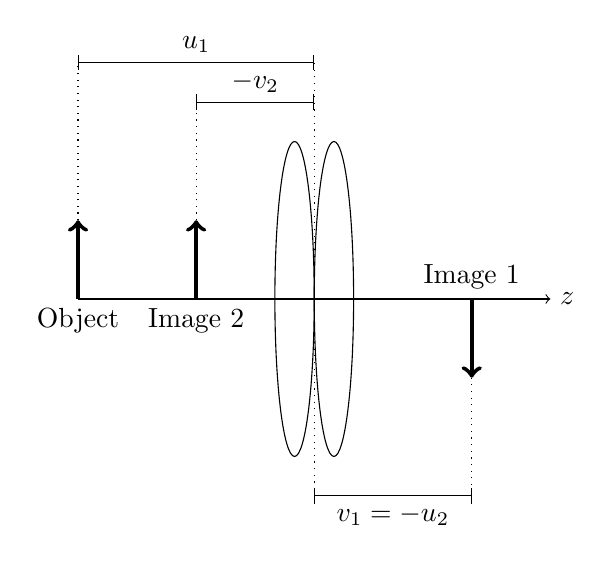
\begin{tikzpicture}
\draw [->] (-3,0) -- (3,0);
\node [right] at (3,0) {\(z\)};
\draw (-0.25,0) ellipse (0.25 and 2);
\draw (0.25,0) ellipse (0.25 and 2);
\draw [->, ultra thick] (-3,0) -- (-3,1);
\draw [->, ultra thick] (-1.5,0) -- (-1.5,1);
\draw [->, ultra thick] (2,0) -- (2,-1);
\node [below] at (-3,0) {Object};
\node [below] at (-1.5,0) {Image 2};
\node [above] at (2,0) {Image 1};
\draw [dotted] (-3,1) -- (-3,3);
\draw [dotted] (-1.5,1) -- (-1.5,2.5);
\draw [dotted] (2,-1) -- (2,-2.5);
\draw [dotted] (0,-2.5) -- (0,3);
\draw [|-|] (-3,3) -- (0,3);
\draw [|-|] (-1.5,2.5) -- (0,2.5);
\node [above] at (-0.75,2.5) {\(-v_2\)};
\node [above] at (-1.5,3) {\(u_1\)};
\draw [|-|] (0,-2.5) -- (2,-2.5);
\node [below] at (1,-2.5) {\(v_1=-u_2\)};
\end{tikzpicture}
\end{center}
The gaussian lens equation:
\[\frac 1u+\frac 1v=\frac 1f\]
Applying the gaussian lens equation for lens 1:
\[\frac{1}{u_1}+\frac{1}{v_1}=\frac{1}{f_1}\]
\[\implies \frac{1}{v_1}=\frac{1}{f_1}-\frac{1}{u_1}\tag{9.1}\]
Applying the gaussian lens equation for lens 2:
\[\frac{1}{u_2}+\frac{1}{v_2}=\frac{1}{f_2}\]
\[\implies \frac{1}{v_2}=\frac{1}{f_2}-\frac{1}{u_2}\]
\[v_1=-u_2\implies\frac{1}{v_2}=\frac{1}{f_2}+\frac{1}{v_1}\]
Substituting in (9.1) gives:
\[\frac{1}{v_2}=\frac{1}{f_2}+\frac{1}{f_1}-\frac{1}{u_1}\]
\[\frac{1}{v_2}+\frac{1}{u_1}=\frac{1}{f_2}+\frac{1}{f_1}\]
Let \(F\) be the effective focus distance of the system:
\[\frac 1F=\frac{1}{v}+\frac{1}{u}\]
\[\implies \frac{1}{F}=\frac{1}{f_1}+\frac{1}{f_2}=\frac{1}{v_2}+\frac{1}{u_1}\]
So the whole system is the same as a single lens with effective focal length \(F\), object distance \(u_1\) and image distance \(v_2\). This shows that focal lengths add in parralel for lenses in contact. This can also be written as powers adding in series as \(P=p_1+p_2\)

\subsection*{Compound microscopes}

Compound microscopes are made from two converging lenses. Image 1 is real and between the two lenses. Image 2 is virtual and further away than the object. You can see the virtual image as you eye is another lens that makes the image real again. The total magnification is given by \(M=M_1M_2\).

\begin{center}
\begin{tikzpicture}
\draw [->] (-5,0) -- (5,0);
\node [right] at (5,0) {\(z\)};
\draw (-2,0) ellipse (0.25 and 2);
\draw (2,0) ellipse (0.25 and 2);
\draw [->, ultra thick] (-5,0) -- (-5,1);
\node [below] at (-5,0) {Object};
\draw [|-|] (-5,2.5) -- (-2,2.5);
\draw [|-|] (-2,2.5) -- (0,2.5);
\draw [|-|] (0,2.5) -- (2,2.5);
\draw [|-|] (2,2.5) -- (5,2.5);
\node [above] at (-3.5,2.5) {\(u_1\)};
\node [above] at (-1,2.5) {\(v_1\)};
\node [above] at (1,2.5) {\(u_2\)};
\node [above] at (3.5,2.5) {\(v_2\)};
\draw [|-|] (-2,-2.5) -- (2,-2.5);
\node [below] at (0,-2.5) {\(d\)};
\end{tikzpicture}
\end{center} 

Applying the gaussian lens equation to both lenses:
\[\frac{1}{v_1}=\frac{1}{f_1}-\frac{1}{u_1}\qquad\frac{1}{v_2}=\frac{1}{f_2}-\frac{1}{u_2}=\frac{1}{f_2}-\frac{1}{d-v_1}\]
We want the rays from the second image to be parallel as this makes the eye relax so the microscope is easier to use. This means that \(v_2\to\infty\):
\[\lim_{v_2\to\infty}\frac{1}{u_2}+\frac{1}{v_2}=\frac{1}{u_2}=\frac{1}{f_2}\implies u_2=f_2\tag{9.2}\]
It can be seen from the diagram that:
\[u_2+v_1=d\implies v_1=d-u_2\]
If we subsititute (9.2) into this we get:
\[v_1=d-f_2\tag{9.3}\]
If we substitute (9.3) into the gaussian lens equation for lens 1 we get:
\[\frac{1}{u_1}=\frac{f_1}-\frac{d-f_2}=\frac{1}{f_1}+\frac{1}{f_2-d}\]
Since we want the waves to end up parallel then we want the object at the focal distance from the lens so \(u_1=F\) so we get that:
\[\frac 1F= \frac{1}{f_1}+\frac{1}{f_2-d}\]

If \(d=0\) then we get the equation for lenses in contact.

\subsection*{Telescopes}

When an object is viewed through a telescope the object is far enough away that we can assume the light rays are parallel. This means that \(u_1\to\infty\). We also want the rays to come out parallel so \(v_2\to\infty\)

The simplest telescope is the gallilean telescope. It is made of a converging and a diverging lens which are set up such that they have there focal point in the same spot. The distance between the lenses is \(d\).
The gaussian lens equation for the first lens as \(u_1\to\infty\):
\[\lim_{u_1\to\infty}\frac{1}{u_1}+\frac{1}{v_1}=\frac{1}{v_1}=\frac{1}{f_1}\implies v_1=f_1\]
The gaussian lens equation for the second lens as \(v_2\to\infty\):
\[\lim_{v_2\to\infty}\frac{1}{u_2}+\frac{1}{v_2}=\frac{1}{u_2}=\frac{1}{f_2}\implies u_2=f_2\]
The magnification is given by:
\[M=-\frac{v_2}{u_1}=\lim_{u_1,v_2\to\infty}=-\frac{\infty}{\infty}\]
This is not a valid answer \Sadey[1.25]


\section{}
If instead we consider the angle \(\vartheta_o\) between the optical axis and the incoming ray which goes through the center of the objective lens. This angle is also made by the ray and the optical axis on the other side of the lens. This forms a right angle triangle between the center of the lens, and the top and bottom of the image. If the image height is \(h\) and the focal length is \(f_o\) then we get the relationship:
\[\tan\vartheta_o=\frac{h}{f_o}\approx\vartheta_o\tag{10.1}\]

If we now consider the angle \(\vartheta_e\) between the optical axis and the ray passing through the center of the eyepiece lens. This angle is part of the right angle triangle fomed between the center of the eyepiece lens, and the top and bottom of the object of the eyepiece lens (which is the image of the objective lens). We get the relationship:
\[\tan\vartheta_e=\frac{h}{f_e}\approx\vartheta_e\tag{10.2}\]

Combining (10.1) and (10.2) we get:
\[\frac{\vartheta_o}{\vartheta_e}\approx\frac{f_e}{f_o}\]

\subsection*{Diffraction}

Diffraction and inteference are a set of phenomona that occur when waves encounter objects about the size of their wavelenght.

In 1D with waves with phase \(\varphi\):
\[y_1+y_2=2A\cos\left(\frac{\varphi}{2}\right)\sin\left(kx-\omega t+\frac{\varphi}{t}\right)\]

\(\cos\left(\frac{\varphi}{2}\right)\) is the phase factor when \(\cos\left(\frac{\varphi}{2}\right)=0\) the waves cancel. In 2D the phase factor is a function of position.

~\makebox[0pt][c]{\rotatebox[origin=c]{90}{( )}} ~These waves are antiphase, they will cancel out, this is called destructive inteference.

~\makebox[0pt][c]{\rotatebox[origin=c]{270}{( (}} ~These waves are in phase, they will add up, this is called constructive inteference.

The difference in path lengths determins how they intefere. For two waves one of which has traveled a distance \(x_1\) and the other \(x_2\) the sum of the two waves is:
\[y_1+y_2=2A\sin\left(k\frac{x_1+x_2}{2}-\omega t\right)\cos\left(k\frac{x_1-x_2}{2}\right)\]

The first term oscilates with time. The second term effects amplitude at different points.
\[I\propto \cos^2\left(k\frac{x_1-x_2}{2}\right)=\cos^2\left(\pi\frac{x_1-x_2}{\lambda}\right)\]

So if the distances differ by an integer number of wavelengths then the waves will be in phase. If it differs by a half integer number of wavelengths then the waves will be out of phase.

\subsection*{Double slit}

\begin{center}
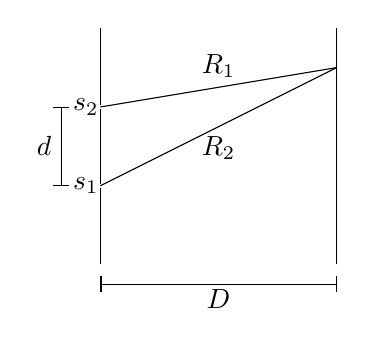
\begin{tikzpicture}[scale=0.5]
\draw (0,0) -- (0,1.95);
\draw (0,2.05) -- (0,3.95);
\draw (0,4.05) -- (0,6);
\node [left] at (0.2,2) {\(s_1\)};
\node [left] at (0.2,4) {\(s_2\)};
\draw [|-|] (-1,2) -- (-1,4);
\node [left] at (-1,3) {\(d\)};
\draw (6,0) -- (6,6);
\draw [|-|] (0,-0.5) -- (6,-0.5);
\node [below] at (3,-0.4) {\(D\)};
\draw (0,2) -- (6,5);
\draw (0,4) -- (6,5);
\node [above] at (3,4.5) {\(R_1\)};
\node [below] at (3,3.5) {\(R_2\)};
\end{tikzpicture}
\end{center}

In general this problem is quite hard to solve but it is simpler when \(D\gg d\) as rays \(R_1\) and \(R_2\) are basically parallel:

\begin{center}
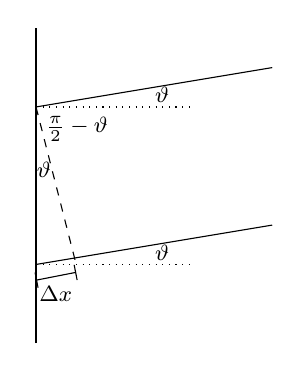
\begin{tikzpicture}
\draw (0,0) -- (0,4);
\draw (0,3) -- (3,3.5);
\draw (0,1) -- (3,1.5);
\draw [dotted] (0,3) -- (2,3);
\draw [dotted] (0,1) -- (2,1);
\draw [dashed] (0,3) -- (0.51,1);
\node at (1.6,3.15) {\footnotesize{\(\vartheta\)}};
\node at (1.6,1.15) {\footnotesize{\(\vartheta\)}};
\node at (0.1,2.2) {\footnotesize{\(\vartheta\)}};
\node [below right] at (0,3) {\footnotesize{\(\frac{\pi}{2}-\vartheta\)}};
\draw [|-|] (0,0.8) -- (0.51,0.9);
\node [below] at (0.25,0.85) {\footnotesize{\(\Delta x\)}};
\end{tikzpicture}
\end{center}

The path difference is \(\Delta x=d\sin\vartheta\). There are maxima at \(\Delta x=m\lambda\) for \(m\in\bb Z\) therefore there are maxima at:
\[m\lambda=d\sin\vartheta\]
Minima are at:
\[\left(m+\frac 12\right)\lambda=d\sin\vartheta\]

\subsection*{Diffraction gratings}

A diffraction grating is a regularly spaced grid of slits, usually engraved on glass.

\begin{center}
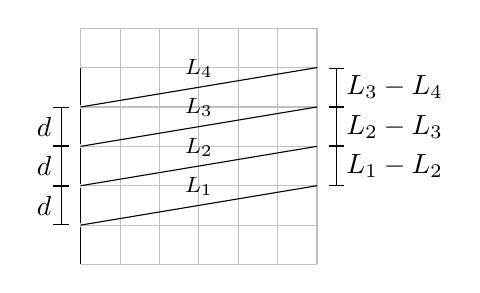
\begin{tikzpicture}[scale=0.5]
\draw [lightgray] (0,0) grid (6,6);
\draw (0,0) -- (0,0.95);
\draw (0,1.05) -- (0,1.95);
\draw (0,2.05) -- (0,2.95);
\draw (0,3.05) -- (0,3.95);
\draw (0,4.05) -- (0,5);
\draw [|-|] (-0.5,1) -- (-0.5,2);
\draw [|-|] (-0.5,2) -- (-0.5,3);
\draw [|-|] (-0.5,3) -- (-0.5,4);
\node [left] at (-0.5,1.5) {\(d\)};
\node [left] at (-0.5,2.5) {\(d\)};
\node [left] at (-0.5,3.5) {\(d\)};
\draw (0,1) -- (6,2);
\draw (0,2) -- (6,3);
\draw (0,3) -- (6,4);
\draw (0,4) -- (6,5);
\draw [|-|] (6.5,2) -- (6.5,3);
\draw [|-|] (6.5,3) -- (6.5,4);
\draw [|-|] (6.5,4) -- (6.5,5);
\node [right] at (6.5,2.5) {\(L_1-L_2\)};
\node [right] at (6.5,3.5) {\(L_2-L_3\)};
\node [right] at (6.5,4.5) {\(L_3-L_4\)};
\node [above] at (3,1.5) {\footnotesize{\(L_1\)}};
\node [above] at (3,2.5) {\footnotesize{\(L_2\)}};
\node [above] at (3,3.5) {\footnotesize{\(L_3\)}};
\node [above] at (3,4.5) {\footnotesize{\(L_4\)}};
\end{tikzpicture}
\end{center}

Making the same assumption as for single slit that \(D\gg d\) so the rays are basically parallel
\[L_1-L_2=L_2-L_3=L_3-L_4=\cdots=d\sin\vartheta\]
\[L_1-L_3=(L_1-L_2)+(L_2-L_3)=d\sin\vartheta+d\sin\vartheta=2d\sin\vartheta\]
In general:
\[L_1-L_{n+1}=nd\sin\vartheta\]
This is generally quite complicated but we know that any two neighbouring rays are in phase as if they where in a double slit experiment. This means that if \(L_1\) and \(L_2\) are in phase then \(L_2\) and \(L_3\) are in phase so by strong induction we know that if \(L_1\) and \(L_2\) are in phase then \(L_1\) is in phase with all other rays. This means that there are maxima at \(m\lambda=d\sin\vartheta\).

The pattern of light depends on \(k\) since \(k=\frac{2\pi}{\lambda}\)
\begin{align*}
m\lambda&=d\sin\vartheta\\
\intertext{For the first fringe:}
\lambda&=d\sin\vartheta\\
\vartheta&\approx\sin\vartheta\\
\lambda&\approx d\vartheta\\
\frac{\lambda}{d}&\approx\vartheta
\end{align*}

This means light will be split into its wavelengths with red light further out than blue. The central fringe will be white.

\section{}
Wavefronts are points/lines/surfaces of constant phase. The exact choice of phase is arbitrary. In 1D it is a series of points traveling with the wave. In 2D it is a line. Wavefronts travel perpendicularly to the energy.

\subsection*{Huygen's principal (HP)}

\begin{displayquote}
Each point of the wavefront acts as a new source of hemispherical ``wavelets" moving in the forward direction
\end{displayquote}

This isn't a fundamental science law but a model. It arrises from a method of solving the underlying wave equation using Green's functions. We can use it to understand diffraction. Each point of the wavefront is creating new wavelets which then create a new wavefront so when a block is discovered the wavefront will create new wavelets which can go around it. The number of wavelets considered isn't important as long as you use enough to get a good picture of what is happening.

It is also possible to derive Snell's law from Huygen's principal:

\begin{center}
\includegraphics[scale=0.3]{HuygensSnellsLaw}
\end{center}

If the wave starts in a medium with refractive index \(n_1\) and travels with velocity \(v_1\) then moves into a medium with refractive index \(n_2\) where it travels with velocity \(v_2\). At time \(t=0\) the first part of the wavefront enters the second medium and creates a wavelet. and at time \(t\) the second ray enters the new medium. By comparing expressions for \(d\) we get Snell's law:
\[\sin \vartheta_1=\frac{v_1t}{d}\]
\[\varphi = \frac{\pi}{2}-\vartheta_2\]
\[\cos\varphi=\frac{v_2t}{d}=\sin\vartheta_2\]
\begin{align*}
d=\frac{v_1t}{\sin\vartheta_1}&=\frac{v_2t}{\sin\vartheta_2}\\
\frac{\sin\vartheta_1}{v_1}&=\frac{\sin\vartheta_2}{v_2}\\
\frac{c\sin\vartheta_1}{v_1}&=\frac{c\sin\vartheta_2}{v_2}\\
n_1\sin\vartheta_1&=n_2\sin\vartheta_2
\end{align*}

It is also possible to derive the double slit inteference pattern by considering two slits that are thin enough that only one wavelet can get through. Since this is a physicaly impossible system we can consider one slit inteference:

\begin{center}
\includegraphics[scale=0.3]{SingleSlit1}
\end{center}

There is a bright fringe at \(P_0\) because if the distance to the screen is much bigger than the slit width then the rays are approximately parallel. Each pair of rays at equal distance apart has the same path difference so it is only necessary to consider one pair:

\begin{center}
\includegraphics[scale=0.3]{SingleSlit2}
\end{center}

As with the double slit cancelation occurs when \(b=\frac a2\sin\vartheta\). First order cancelation \(\frac{\lambda}{2}=b=\frac a2\sin\vartheta\) So there are minima at \(\lambda=a\sin\vartheta\). So for the complete single slit:
\[b=x\sin\vartheta\]
\begin{align*}
A_x &= A_0\sin(k(D-b)-\omega t)\\
&= A_0\sin(kD-kx\sin\vartheta-\omega t)\\
&= A_0[\sin(kD-\omega t)cos(kx\sin\vartheta)-\cos(kD-\omega t)\sin(kx\sin\vartheta)]
\end{align*}
Where \(x\) is the distance from the center of the slit.

\section{}

A crystal is a solid with a repeating molecular structure. It has planes of molecules:

\begin{center}
\includegraphics[scale=0.2]{CrystalPlanes}
\end{center}

The distance between planes is approximately \(10^{-10}\) which is about the same as the wavelength of x-rays therefore x-rays will defract in a crystal. The different layers of the crystal act as a diffraction grating.

\subsection*{X-ray crystalography - single crystal}

When an x-ray is incident on a crystal if it hits a molecule a diffuse reflection occurs. Most of the reflected rays will cancel leaving rays at only specific angles with perfecly constructive inteference. If we consider only the rays that don't cancel:

\begin{center}
\includegraphics[scale=0.4]{CrystalReflection}
\end{center}

The two rays leaving are close enough to intefere. The path difference \(\Delta\) is given by:
\[\Delta = 2L=2d\sin\vartheta\]
So the inteference is constructive if:
\[m\lambda=2d\sin\vartheta\text{ for }m\in\bb Z\]
Note that \(\vartheta\) is not the angle of incidence \(\vartheta_i\) but rathter \(\vartheta = \frac{\pi}{2}-\vartheta_i\).

This is Bragg's law

Each plane has different spacing so there are different angles of reflection depending on the angle the light is shone.

\subsection*{X-ray crystalography - powdered crystal}

In reality a powederd crystal is used. This results in a circular diffraction pattern.

\begin{center}
\includegraphics[scale=0.2]{CrystalPowder}
\end{center}

\subsection*{Thin Film Inteference}

A thin film will cause light reflecting off of the two edges of the film to intefere with itself. We imagine light normal to the surface of the film. The path difference length is affected by three factors:
\begin{itemize}
\item Physical length difference
\item Refractive index (\(n_{\text{film}}>n_{\text{air}}\))
\item Phase shift on reflection from surface of higher refractive index by \(\si{\pi rad}\) 
\end{itemize}
This results in a phase difference \(\Delta\varphi\) for a film thickness \(L\)
\[\Delta\varphi=2kL-\pi\]
The first term \(2kL\) is due to the physical length difference. The second term \(\pi\) is due to the reflection. \(k\) is the wavenumber in the film. \(k = k_{\text{film}}=\frac{2\pi}{\lambda_{\text{film}}}\). \(\omega\) is constant and \(v\) changes.
\[\lambda_{\text{film}}=\frac{\lambda_{\text{air}}}{n_{\text{film}}}\]
\[\implies\Delta\varphi=\frac{4\pi nL}{\lambda}-\pi\]
Constructive inteference occurs if \(\Delta\varphi=2m\pi\) hence \(2L = \left(m+\frac 12\right)\frac{\lambda}{n}\) and destructive inteference occurs if \(\Delta\varphi=(2m+1)\pi\) hence \(2L = \frac{m\lambda}{n}\) for \(m\in\bb Z\)

\subsection*{Uses of interference}

\begin{itemize}
\item Interferometer - A genereal class of tools using path difference for measurement
\item Radio interferometry - Multiple radiotelescopes aproximately \SI{10}{km} apart with correlated ouputs that act as a \SI{10}{km} wide telescope. It can only see small stuff as \(\sin\vartheta\propto\frac{\lambda}{d}\)
\item The Michelson-Morley experiment (which shows there is no aether)
\item LIGO (which discovered gravitational waves)
\end{itemize}
